\documentclass[main.tex]{subfiles}
\begin{document}

\chapter{Evaluation}

In diesem kapitel werden zuvor ausgewählte algorithmen einheitlich verglichen und die resultierenden ergebnisse ausgewertet.

\section{Evaluation Protocol}

To determine the feasibility of performing real-time plane detection, we need to conduct experiments with the selected algorithms.

Another important factor for comparability is the data set, on which the experiments are conducted on.
Because each publication from the presented algorithms uses a different data set for its evaluation, we cannot objectively select an algorithm to be the "best".
Furthermore, to the best of our knowledge, there is no data set, that contains an incrementally growing and unordered point cloud with corresponding ground truth.

Thus, we first evaluate the algorithms on a dataset while excluding the temporal component. We do this by performing plane detection on whole point clouds, rather than
incrementally growing ones.

We then perform experiments, this time including the temporal component, by performing calculations at each time step and evaluating them individually.

Lastly, through comparison, as well as analysis of those different experiments, a statement will be given as to whether and how well plane detection is
possible in real-time.

For the evaluation of a given dataset, by comparing the test results with the ground truth, we took inspiration from \citeauthor{Araújo_Oliveira_2020} \citedate{Araújo_Oliveira_2020},
especially their \textit{Results} chapter.


\subsection{Metrics}
To quantitatively evaluate an algorithm's performance, we calculate the precision, recall and the f1 score.
First, we regularize the original point cloud to reduce complexity and furthermore to avoid proximity bias, because of the inverse relationship
between distance to sensor and cloud density. This regularization is obtained through voxelization of the point cloud.\\
With this voxel grid, we can now calculate corresponding sets of voxels for each point cloud representing a plane.
In the next step, we compare our planes from the ground truth with the planes obtained from an algorithm to obtain a list of corresponding pairs
of ground truth and found planes.\\
A grund truth plane $p_{gt_i}$ is marked as \textit{detected}, if any plane from the list of found planes achieves a voxel overlap of $\geq 50\%$.
With this list of correspondences, we calculate precision, recall and the f1-score as explained in the following.
For a given ground truth plane $p_{gt_j}$ and a corresponding found plane $p_{a_k}$ we can sort a given voxel $v_i$ into the categories
\textit{True Positive(TP), False Positive(FP) and False Negative(FN)} as follows.
$$v_i \in p_{gt_j} \land v_i \in p_{a_k} \Rightarrow v_{i} \in TP$$
$$v_i \in p_{gt_j} \land v_i \notin p_{a_k} \Rightarrow v_{i} \in FN$$
$$v_i \notin p_{gt_j} \land v_i \in p_{a_k} \Rightarrow v_{i} \in FP$$
% TODO not needed right? $$v_i \notin p_{gt_j} \land v_i \notin p_{a_k} \Rightarrow v_{i} \in TN$$  , True Negative(TN)} 

With those four rules, we can calculate the precision, recall and F1 score like this:
$$Precision = \frac{|TP|}{|TP|+|FP|}$$
$$Recall = \frac{|TP|}{|TP|+|FN|}$$
$$F1 = 2 \cdot\frac{Precision\cdot Recall}{Precision + Recall}$$

Aside from the accuracy, we also need to compare the time each algorithm needs to find its respective set of planes.
For that, we measure the time spent in the plane detection phase, excluding any preprocessing or postprocessing steps.
To measure the detection time, we log the exact times before and after calculations and write the difference to a file.\\


\subsection{Dataset}
To evaluate each plane detection algorithm on even grounds, we select the Stanford Large-Scale Indoor Spaces 3D Dataset(S3DIS)\cite{2017arXiv170201105A}. The Dataset had been recorded in three different buildings,
which then were divided into six distinct areas. Those six areas include a total of 270 different types of rooms, e.g. offices, hallways, WCs and two auditoriums to name a few.\\
Each room has a complete unstructured point cloud in form of a list of XYZ values, as well as a list of annotated files representing semantically different objects that can be found in this point cloud
of the room.
Since our focus lies not on 3D semantic segmentation, we manually select planar regions using CloudCompare\footnote{\href{https://cloudcompare.org/}{https://cloudcompare.org/}}, obtaining a list of sub-clouds.

\begin{table}[]
    \centering
    \begin{tabular}{c|c|c|c|c|c|c|c}
        \hline
        Scene Categories & Area\_1 & Area\_2 & Area\_3 & Area\_4 & Area\_5 & Area\_6 & TOTAL \\ \hline
        office           & 31      & 14      & 10      & 22      & 42      & 37      & 156   \\ \hline
        conference room  & 2       & 1       & 1       & 3       & 3       & 1       & 11    \\ \hline
        auditorium       & -       & 2       & -       & -       & -       & -       & 2     \\ \hline
        lobby            & -       & -       & -       & 2       & 1       & -       & 3     \\ \hline
        lounge           & -       & -       & 2       & -       & -       & 1       & 3     \\ \hline
        hallway          & 8       & 12      & 6       & 14      & 15      & 6       & 61    \\ \hline
        copy room        & 1       & -       & -       & -       & -       & 1       & 2     \\ \hline
        pantry           & 1       & -       & -       & -       & 1       & 1       & 3     \\ \hline
        open space       & -       & -       & -       & -       & -       & 1       & 1     \\ \hline
        storage          & -       & 9       & 2       & 4       & 4       & -       & 19    \\ \hline
        WC               & 1       & 2       & 2       & 4       & 2       & -       & 11    \\ \hline
        TOTAL            & 45      & 39      & 24      & 49      & 55      & 53      & 272   \\
    \end{tabular}
    \caption{S3DIS Disjoint Space Statistics}
    \label{tab:stanfordStats}
\end{table}

\subsection{Real-Life Test}
We record an incrementally growing data set in the Faculty of Computer Science at Otto-von-Guericke University Magdeburg.
Running \textit{realsense-ros} and holding our cameras, we walk through different parts of the building, scanning to the best of our ability.
We save each incremental map update to a file for later usage.

We create a set of ground truth planes $gt_{end}$for only the most recent update, e.g., for the entire recording.

To prepare for the evaluation of a map $m_t$ at a given time $t$, we crop all planes in $gt_{end}$ by removing all points that are not present in $m_t$. 
We speed up this expensive process by employing a KD-Tree neighbor search with a small search radius since we only need to know whether a certain point is present or not. 
Furthermore, we remove planes from the ground truth, if the number of included points falls short of a threshold.

\begin{figure}[!ht]
	\centering
	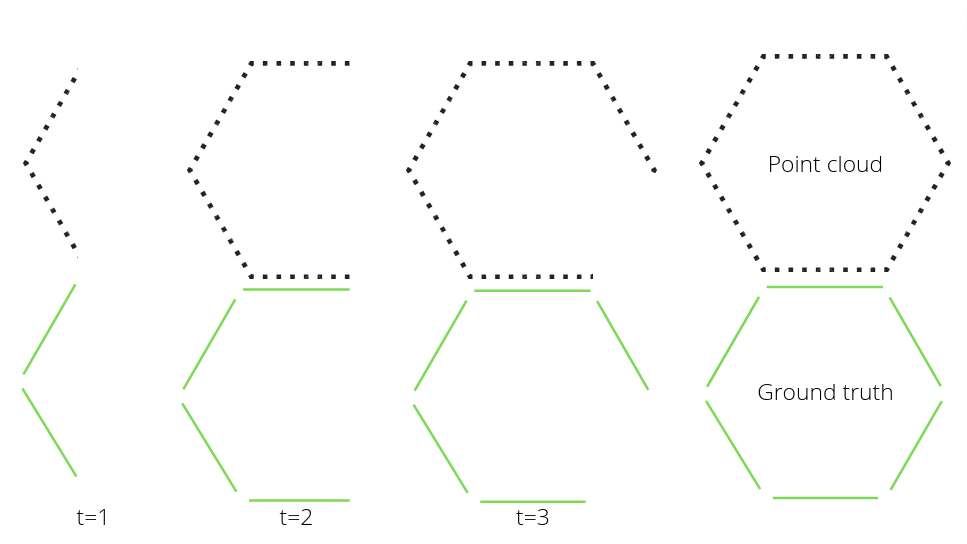
\includegraphics[width=15 cm]{images/dynamic_eval.png}
\end{figure}


\section{Results}

\subsection{Results Dataset}


\paragraph*{Area 1}
Hier sind die Ergebnisse von Area 1:

\begin{figure}
	\centering
	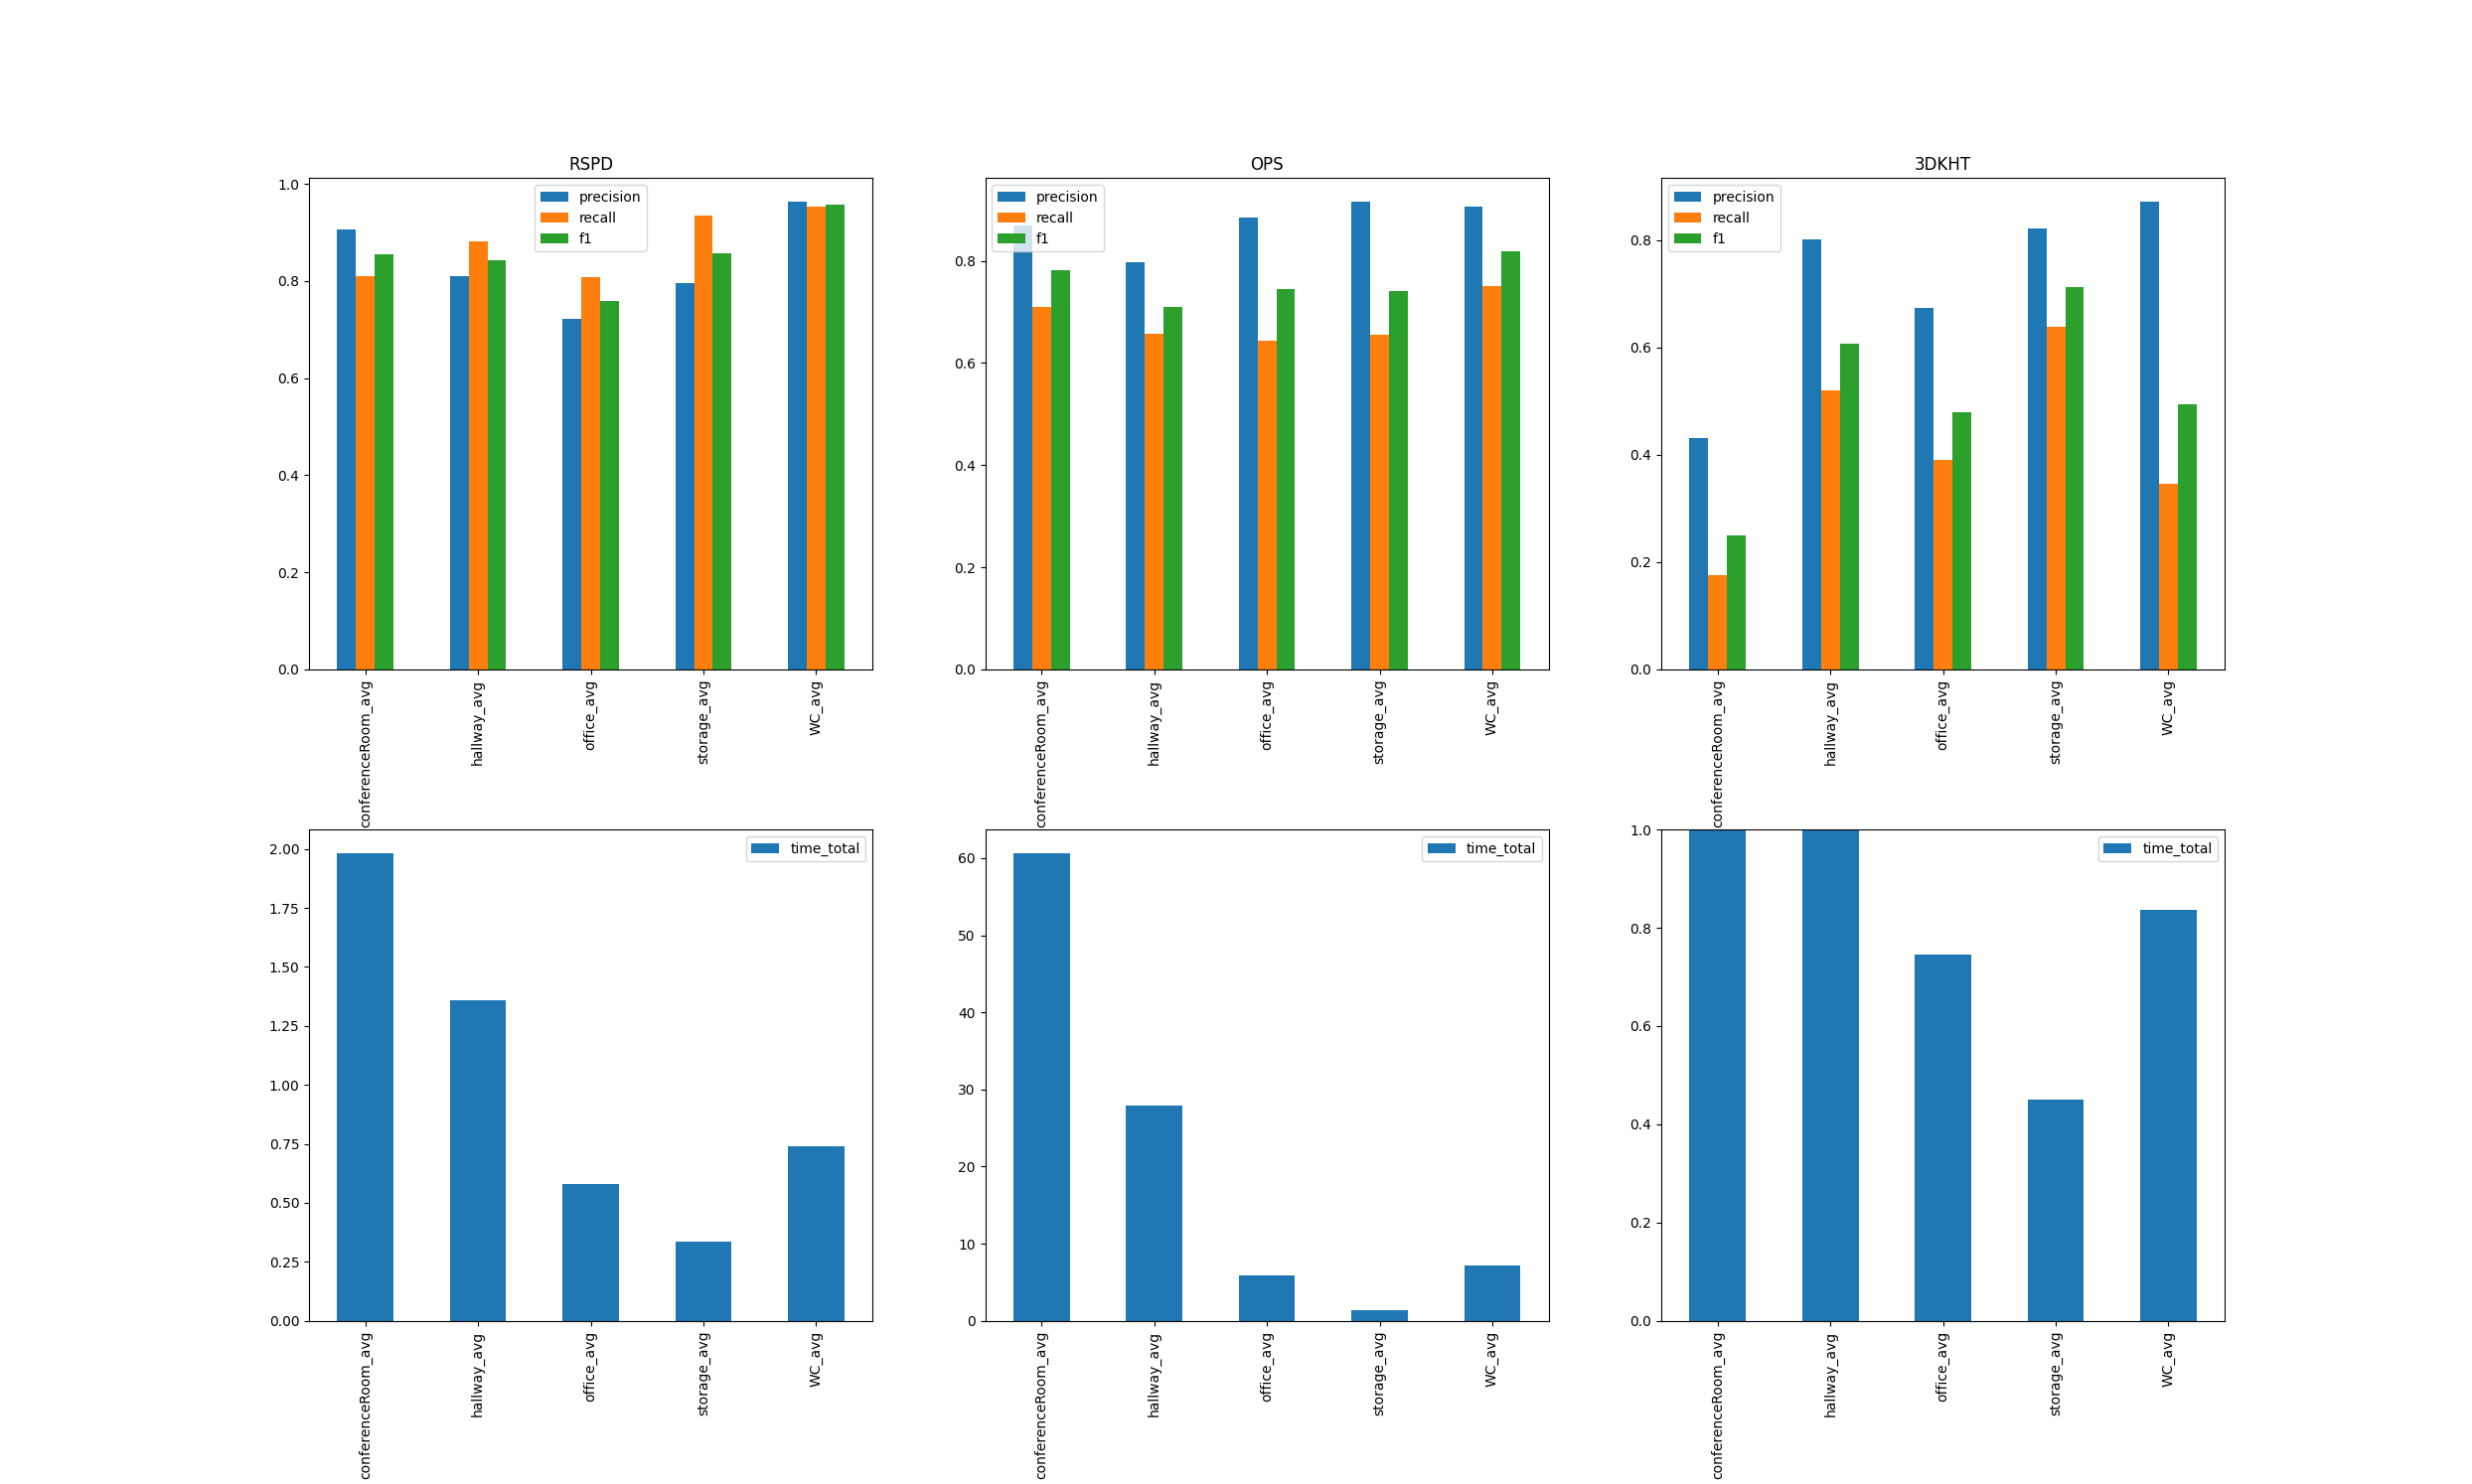
\includegraphics[width=15 cm]{images/area_1_ohne_kht.png}
	\label{fig:area1}
    \caption{Results Area 1}
\end{figure}

\paragraph*{Area 2}
Hier sind die Ergebnisse von Area 2:

\begin{figure}
	\centering
	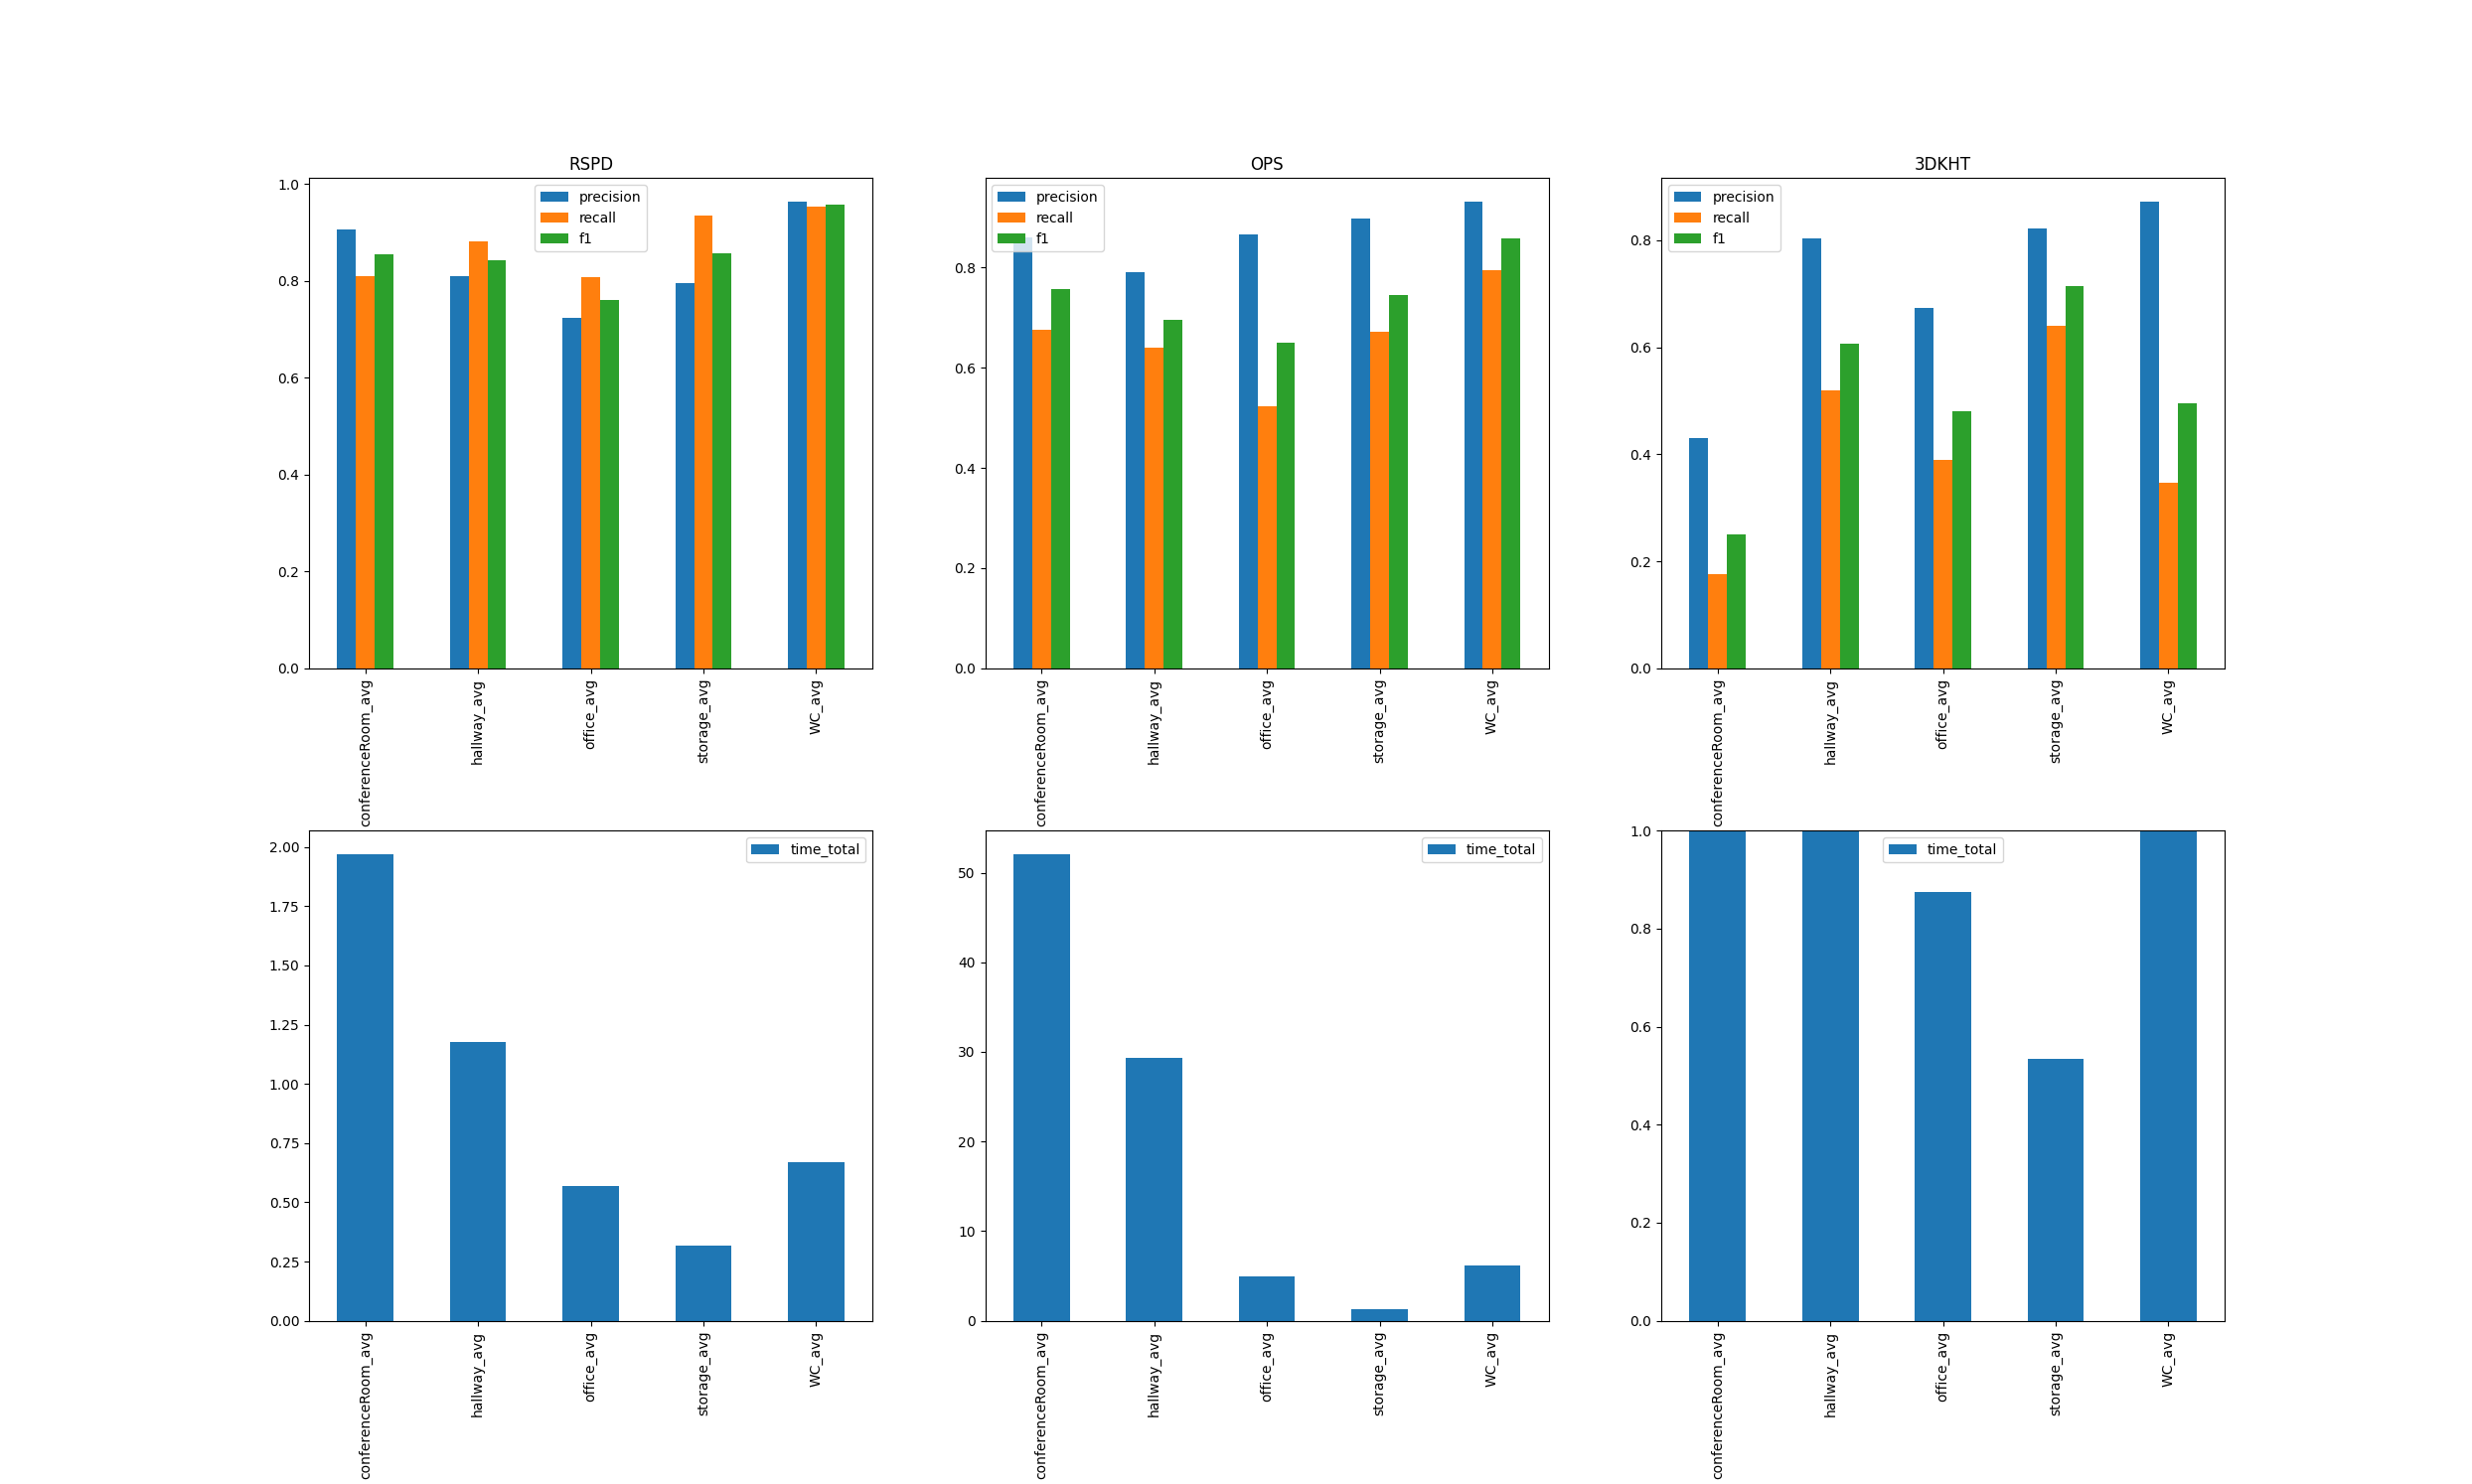
\includegraphics[width=15 cm]{images/area_2_ohne_kht_ohne_audi.png}
	\label{fig:area2}
    \caption{Results Area 2}
\end{figure}

\paragraph*{Area 3}
Hier sind die Ergebnisse von Area 3:

\begin{figure}[!ht]
	\centering
	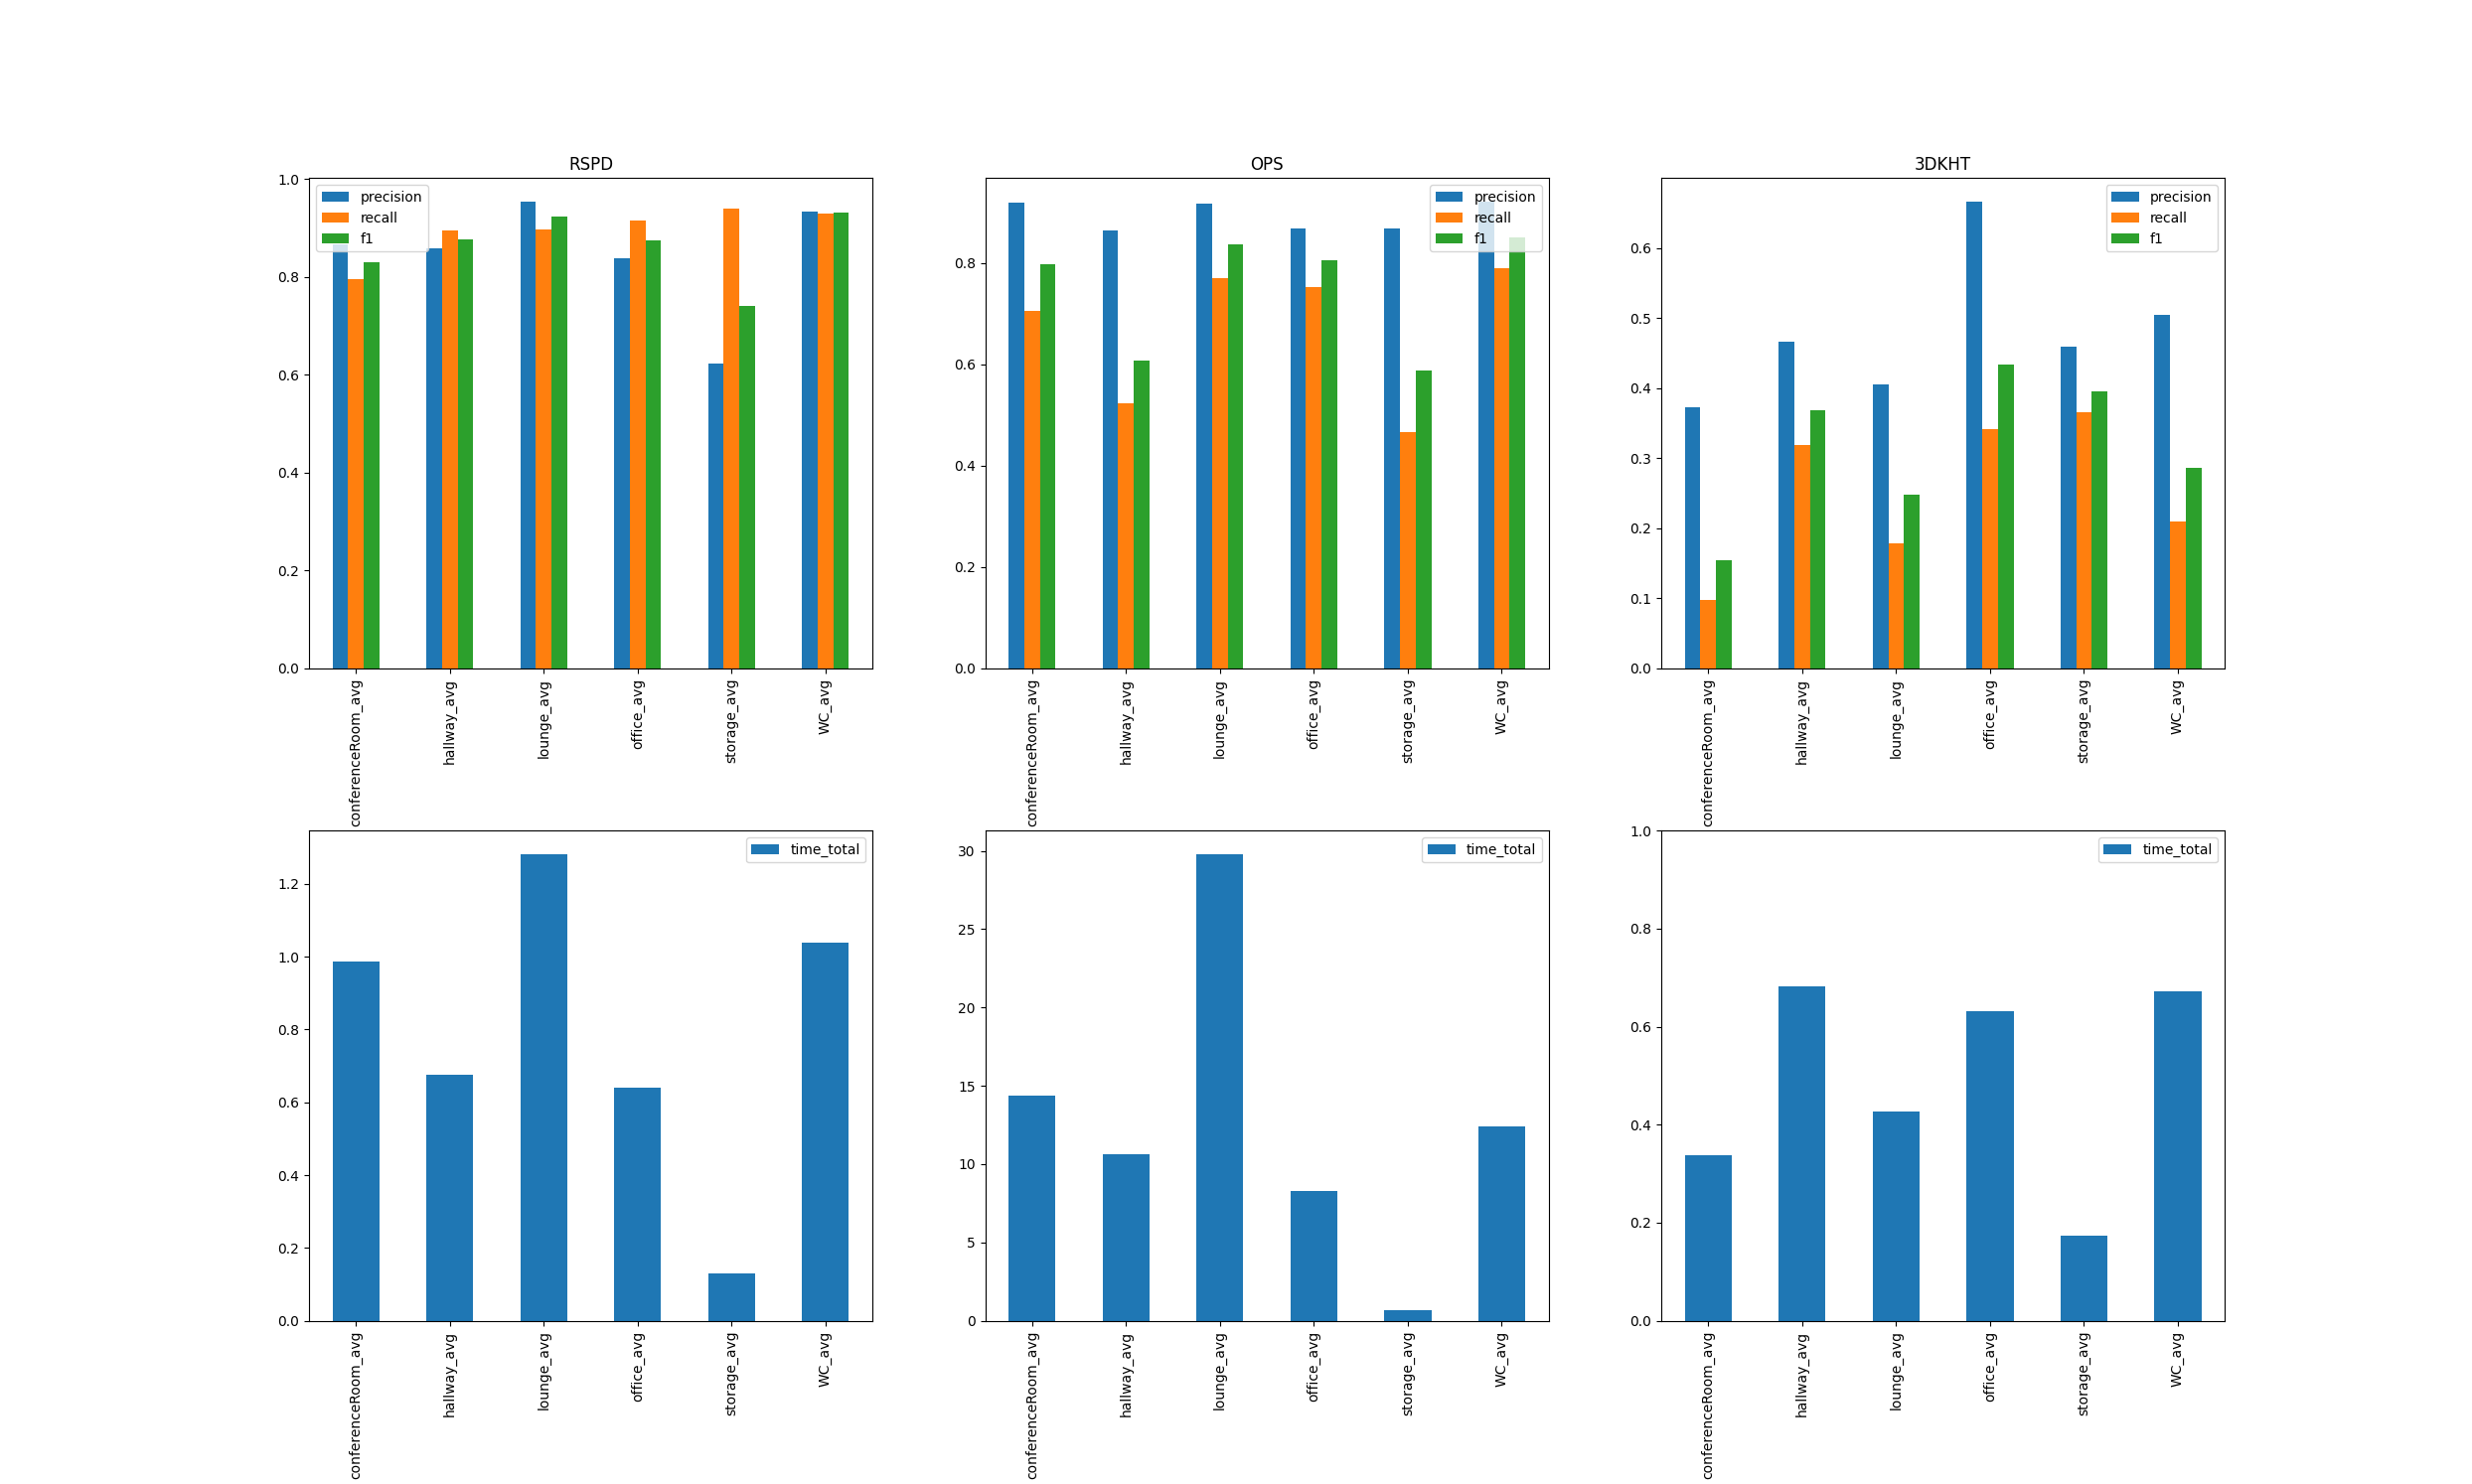
\includegraphics[width=15 cm]{images/area_3_ohne_kht.png}
	\label{fig:area3}
    \caption{Results Area 3}
\end{figure}

\paragraph*{Area 4}
Hier sind die Ergebnisse von Area 4:

\begin{figure}
	\centering
	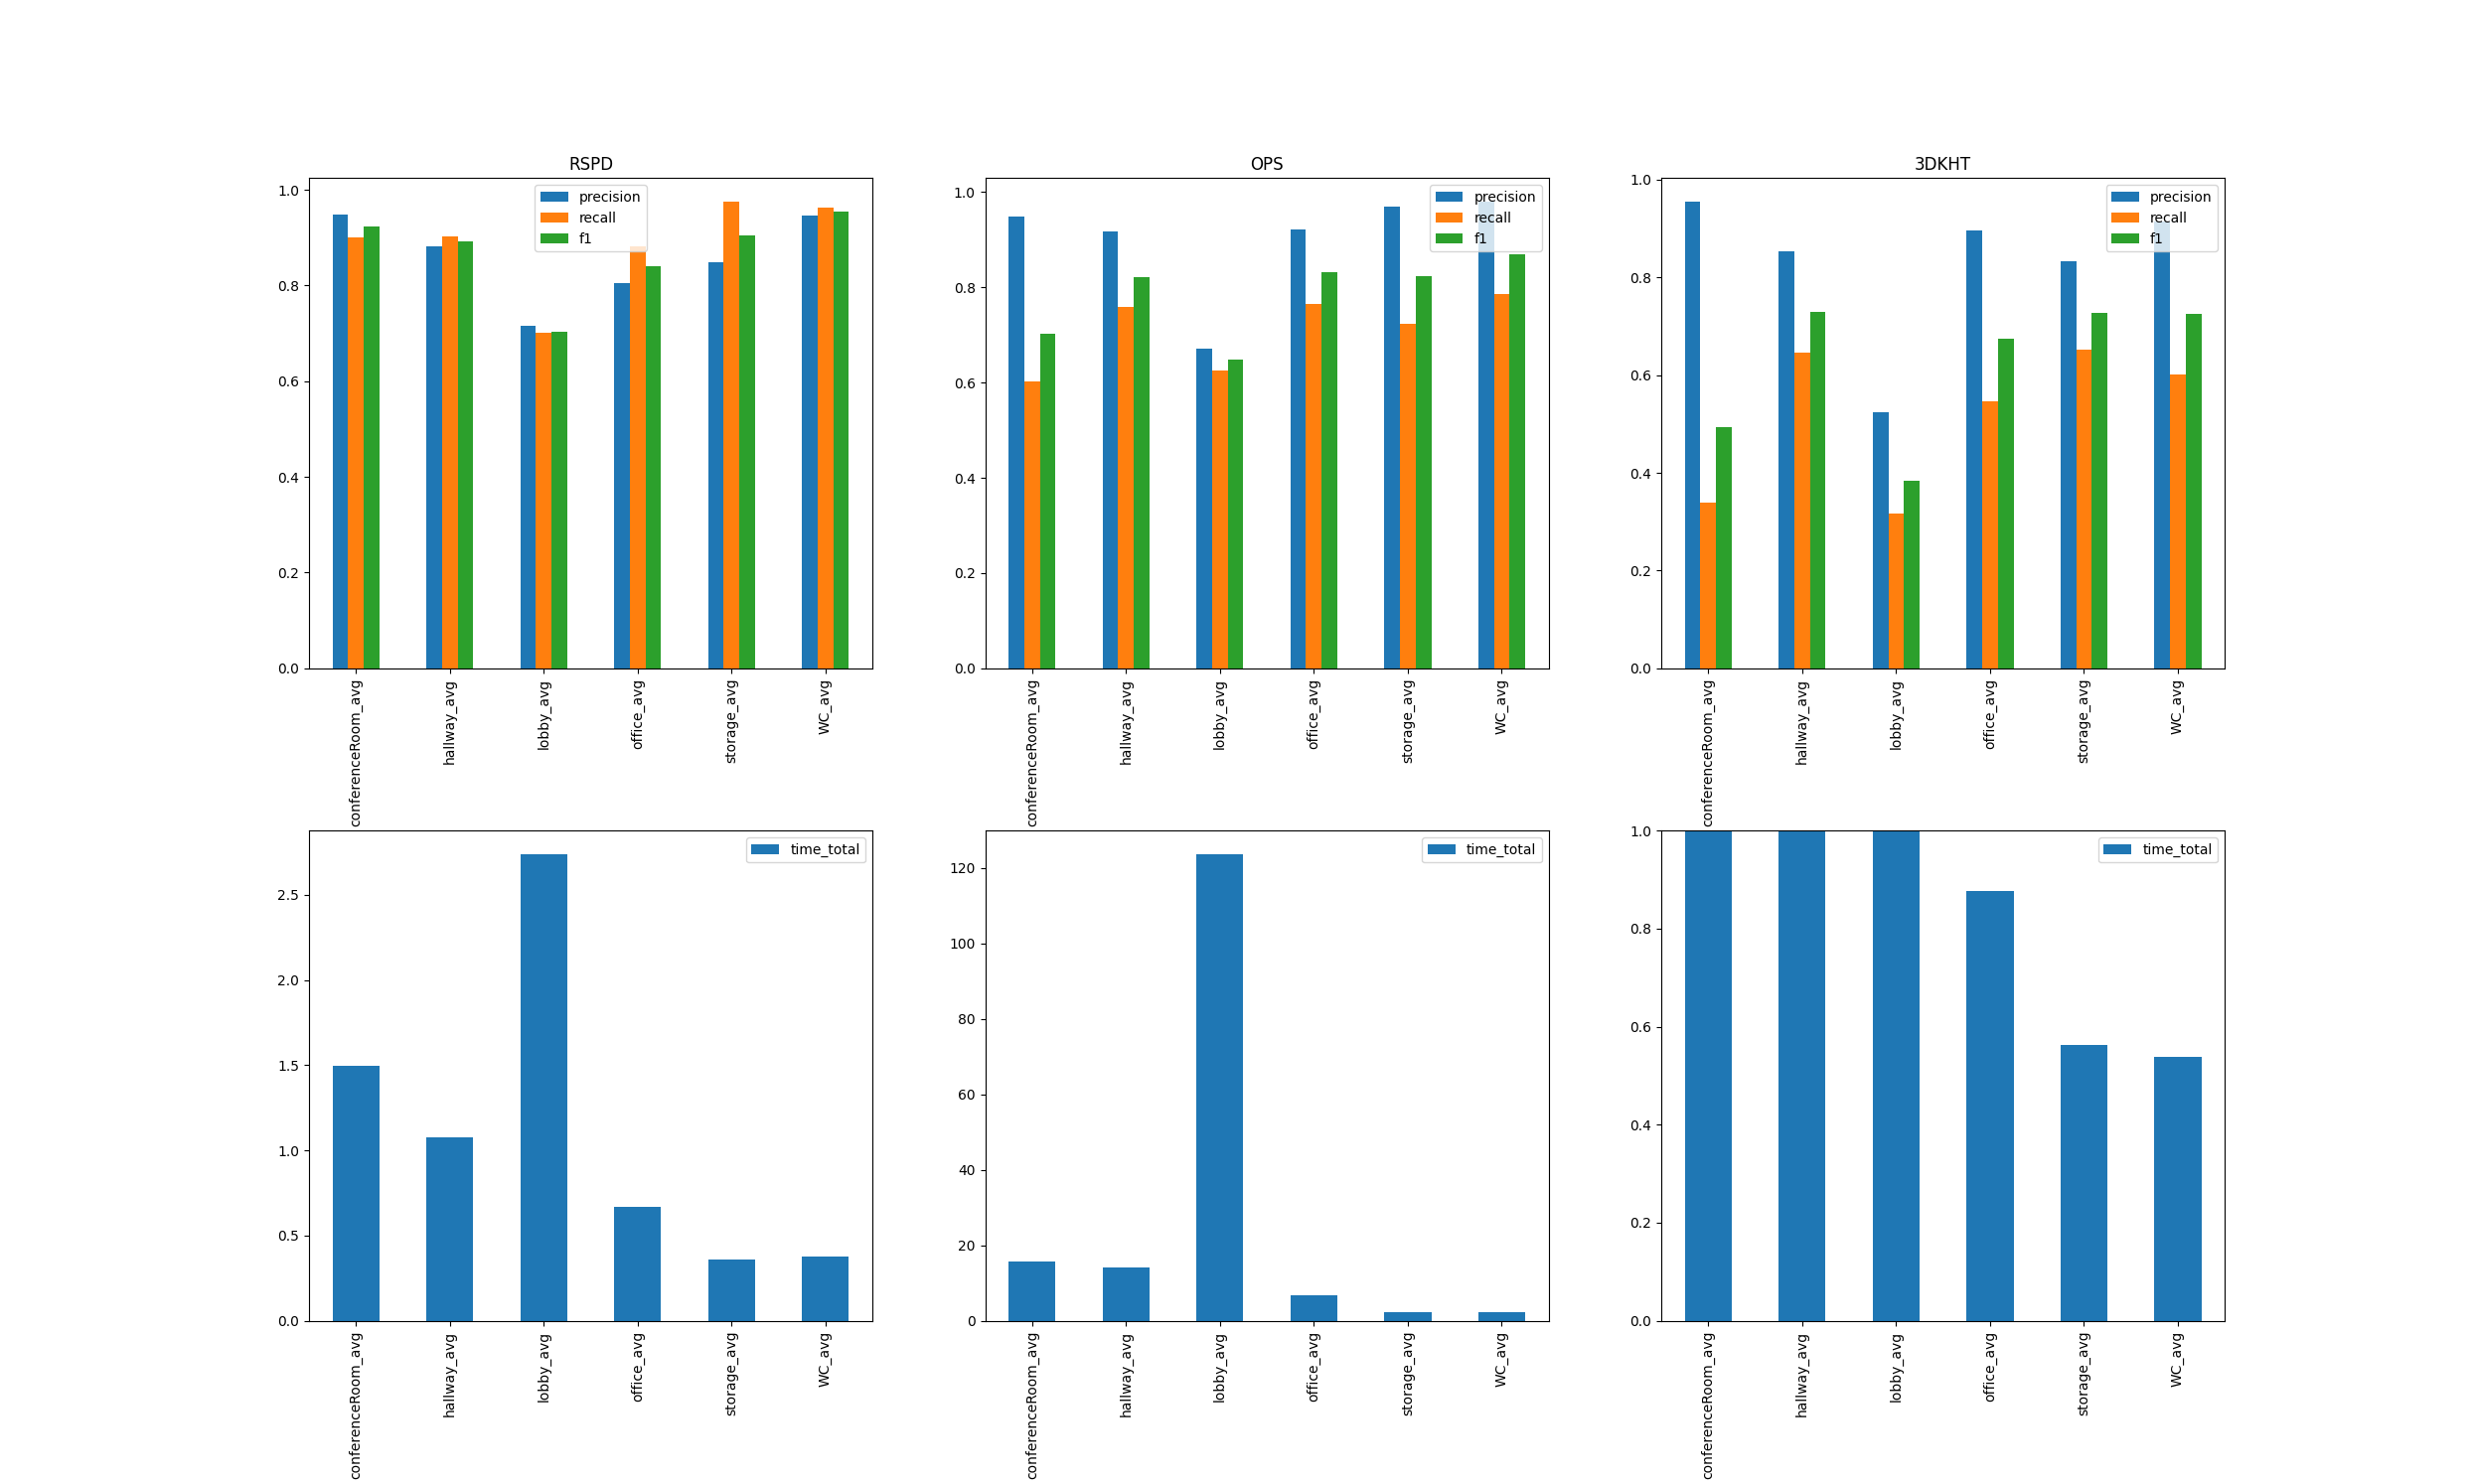
\includegraphics[width=15 cm]{images/area_4_ohne_kht.png}
	\label{fig:area4}
    \caption{Results Area 4}
\end{figure}

\subsection{Results Real-Life Test}

Hier sind die Ergebnisse:


\end{document}